% !TEX root = knottedMain.tex
\documentclass[varwidth=\maxdimen]{standalone}

\usepackage{mathtools,amssymb,mathrsfs,dutchcal,upgreek,faktor,accents,etoolbox,multicol}
\usepackage[dvipsnames]{xcolor}
\definecolor{mygreen}{RGB}{	8,156,79 }
\usepackage{tikz,tikz-cd}
\usetikzlibrary{patterns,knots,arrows.meta,decorations.markings}
\tikzset{>={Straight Barb[scale=0.85]}}
\tikzcdset{
  cells={font=\everymath\expandafter{\the\everymath\displaystyle}},
  arrow style=tikz,
  diagrams={>={Straight Barb[scale=0.85]}},
  every label/.append style = {font = \small}
}


\begin{document}

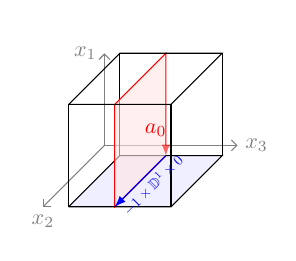
\begin{tikzpicture}[scale=1.3,every node/.style={scale=0.8}]
    \clip (-1.15,-1) rectangle (1.2,1);
    \draw[->,black!50] 
        (-0.4,-0.15) -- (-0.4,0.75) node[left]{$x_1$};
    \draw[->,black!50] 
        (-0.4,-0.15) -- (-1,-0.75) node[below]{$x_2$};
    \draw[->,black!50] 
        (-0.4,-0.15) -- (0.9,-0.15) node[right]{$x_3$};


    \draw
        (-0.25,-0.25) rectangle (0.75,0.75);
    \fill[blue!10,fill opacity=0.6,draw=black]
        (-0.75,-0.75) -- (0.25,-0.75) -- 
        (0.75,-0.25) -- (-0.25,-0.25) -- (-0.75,-0.75);
    \fill[red!10,fill opacity=0.6,draw=red,-latex]
          (0.2,-0.25) -- (-0.3,-0.75) -- (-0.3,0.25) --
         (0.2,0.75) -- (0.2,-0.25);
    \fill[white,fill opacity=0,draw=black]
        (-0.75,0.25) -- (0.25,0.25) -- 
        (0.75,0.75) -- (-0.25,0.75) -- (-0.75,0.25);

    \draw (-0.75,-0.75) rectangle (0.25,0.25);

    \draw  (0.1,0) node[red]{$a_0$};
    \draw[blue,-latex] (0.2,-0.25) -- (-0.3,-0.75) node[right,pos=0.4,below,scale=0.65,rotate=45]{$-1\times\mathbb{D}^1\times0\,$}; 
\end{tikzpicture}

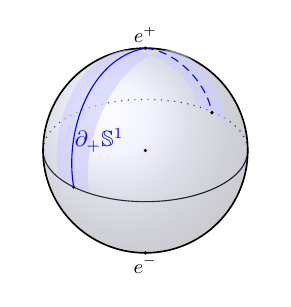
\begin{tikzpicture}[scale=1.3,every node/.style={scale=0.8},even odd rule]
\clip (-1.15,-1.25) rectangle (1.15,1.2);
    \draw[black] (-1,0) arc (180:360:1cm and 0.5cm);
    \draw[black,dotted] (-1,0) arc (180:0:1cm and 0.5cm);
    \shade[ball color=blue!20!,opacity=0.3] (0,0) circle (1cm);
    \draw[black,semithick] (0,0) circle (1cm);
    \fill (0,0) circle (0.5pt) ;


    \fill[blue!20,opacity=0.6]
        (0.5,0.45) to[in=0,out=100,distance=0.3cm]  (-0.2,0.98) to[out=-170,in=100,distance=0.5cm] (-0.85,-0.26) to[out=-20,in=170,distance=0.1cm] (-0.55,-0.4)
        to[in=-170,out=100,distance=0.5cm] (0.2,0.98)  to[out=0,in=100,distance=0.3cm]  (0.8,0.3) to[in=-20,out=170,distance=0.1cm] (0.5,0.45) ;
            
    \draw[blue]
        (0,1) to[out=-170,in=100,distance=0.55cm] (-0.7,-0.358) ;
    \draw[blue,densely dashed]
        (0,1) to[out=-5,in=100,distance=0.3cm] 
        (0.65,0.37);

    \fill
        (0,1)   circle (0.5pt) 
                node[above=-1pt]{\small$e^+$}
        (0,-1)  circle (0.5pt) 
                node[below=-2pt]{\small$e^-$}
        (-0.7,-0.358) circle (0.5pt)
        (0.65,0.37) circle (0.5pt)
        (-0.45,0.1) node[blue]{$\partial_+\mathbb{S}^1$}
        ;
    
\end{tikzpicture}

\end{document}